\documentclass[12pt]{beamer}
\usetheme{Boadilla}
\usepackage{booktabs}
\usepackage{multirow}
\usepackage{enumitem}
\usepackage{tikz}

\newcommand{\E}{\mathbb{E}}
\usefonttheme{professionalfonts}
\usepackage{pgfplots}
\pgfplotsset{compat=1.18}
\renewcommand{\arraystretch}{1.25}
\usetikzlibrary{trees}
\title[ECON2843]{Lecture 17}
\subtitle{Part 3 Estimation and Hypothesis Test}
\date{}
\usepackage{amsmath,amssymb,mathtools,wasysym}
\begin{document}
	\begin{frame}
		\titlepage
	\end{frame}
	\begin{frame}
		\vspace{1cm}
		\centering
		{\color{blue}\large $F$-distribution}
	\end{frame}

	\begin{frame}
		\frametitle{$F$-distribution}
		
		\begin{itemize}[label={\color{blue}$\blacktriangleright$}]
			\item The null distribution of this $F$-statistic is an $F$-distribution with $n_1 - 1$ numerator degrees of freedom and $n_2 - 1$ denominator degrees of freedom.
			\item The $F$-distribution is a special continuous distribution:
			\begin{itemize}[label={\color{blue}$\blacktriangleright$}]
				\item It has two parameters called the numerator degrees of freedom and the denominator degrees of freedom.
				\item $F$-tables give critical values that cut off probability $A$ in the upper tail.
				\item There is a different table for each value of $A$.
				\item Rows and columns display the degrees of freedom.
			\end{itemize}
		\end{itemize}
		
	\end{frame}
		\begin{frame}
		\frametitle{$F$-distribution}
\centering
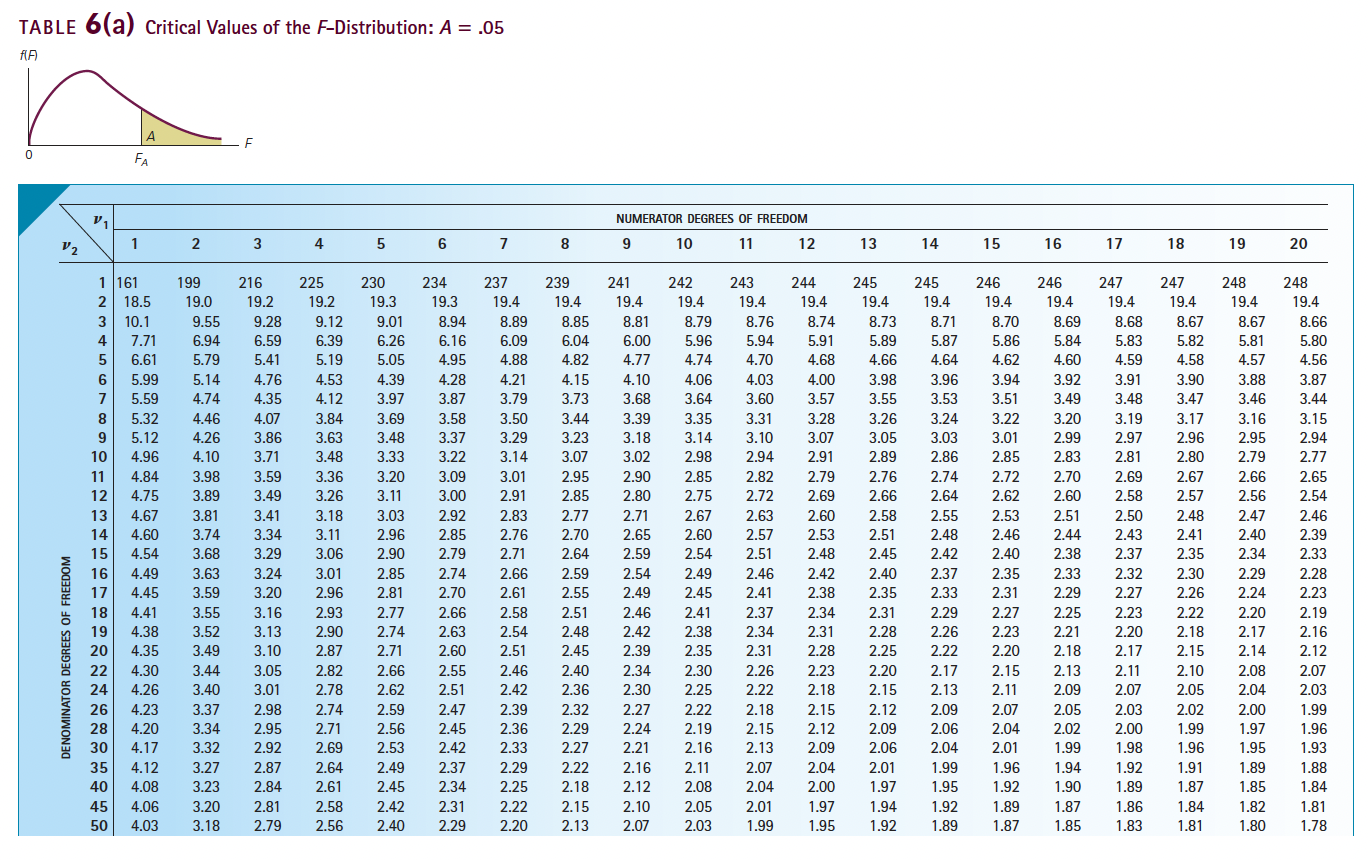
\includegraphics[width=11cm]{fstat.png}	
		
	\end{frame}
	\begin{frame}
		\frametitle{Population Variances are Unknown}
		\framesubtitle{Testing Equality of Variances}
		
		\begin{itemize}[label={\color{blue}$\blacktriangleright$}]
			\item Decision rule:
			\begin{itemize}[label={\color{blue}$\blacktriangleright$}]
				\item Compare the $F$-statistic to the appropriate $F$-distribution.
				\item For a given value of $\alpha$, reject the null hypothesis if
				
				\[F < F_{1-\frac{\alpha}{2},n_1-1,n_2-1} \text{ or } F > F_{\frac{\alpha}{2},n_1-1,n_2-1}\]
				
				where $F_{1-\frac{\alpha}{2},n_1-1,n_2-1}$ and $F_{\frac{\alpha}{2},n_1-1,n_2-1}$ are the critical values that cut off $100 \left(\frac{\alpha}{2}\right)\%$ in the lower and upper tails, respectively, of the appropriate $F$-distribution.
				\item But the tables don't give us the lower cut-off values.
				\item Special trick for doing test...
			\end{itemize}
		\end{itemize}
		
	\end{frame}
		\begin{frame}
		\frametitle{Population Variances are Unknown}
		\framesubtitle{Testing Equality of Variances}
\centering
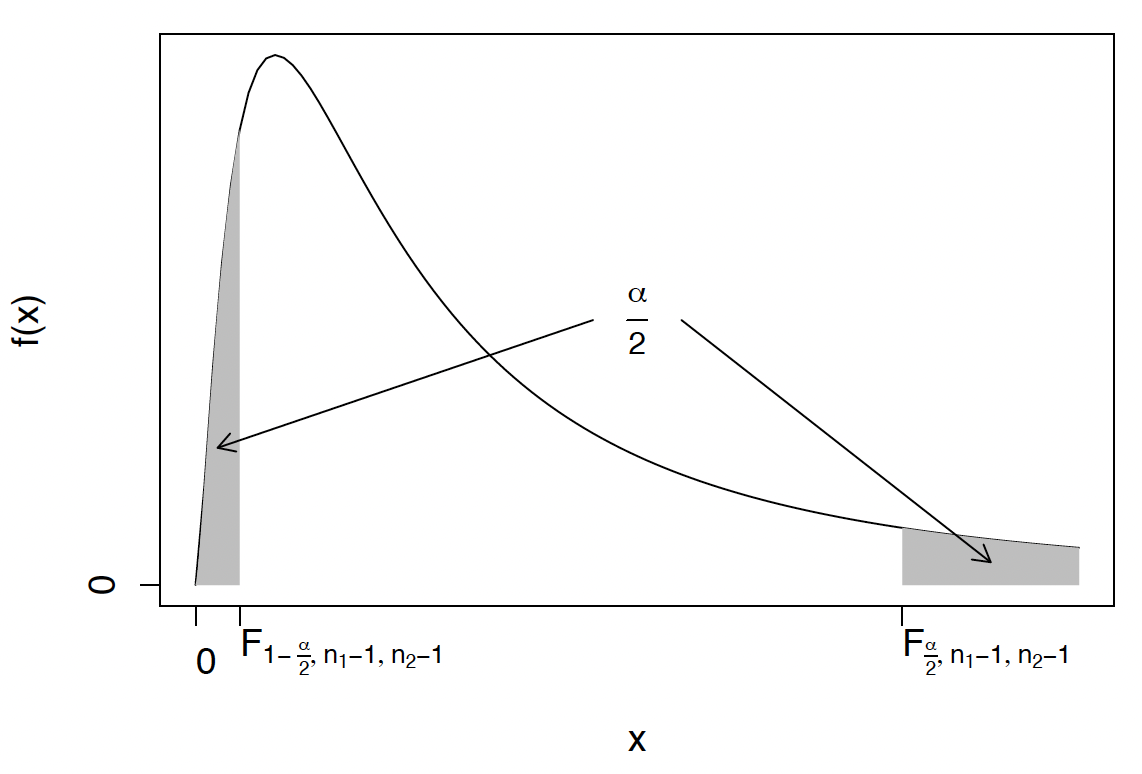
\includegraphics[width=10cm]{eqvar.png}	
	\end{frame}
	\begin{frame}
		\frametitle{Population Variances are Unknown}
		\framesubtitle{Testing Equality of Variances}
		
		
		\[
		F = \frac{s_1^2}{s_2^2}
		\]
		
		
		\begin{itemize}[label={\color{blue}$\blacktriangleright$}]
			\item The labeling of sample 1 and sample 2 is arbitrary, so always put the larger sample variance on top.
			\item Then our $F$-statistic will always be larger than 1, and we only have to look up the upper cut-off and reject $H_0$ at significance level $\alpha$ whenever 
			\[F > F_{\frac{\alpha}{2},n_1-1,n_2-1}.\]
		\end{itemize}
		
	\end{frame}
	\begin{frame}
		\frametitle{Population Variances are Unknown}
		\framesubtitle{Testing $\mu_1 - \mu_2$ when $\sigma_1^2 = \sigma_2^2$}
		
		\begin{itemize}[label={\color{blue}$\blacktriangleright$}]
			\item Hypotheses:
			\[
			\begin{aligned}
				H_0 &: \mu_1 - \mu_2 = D_0 \\
				H_1 &: \mu_1 - \mu_2 (\neq, <, >) D_0
			\end{aligned}
			\]
			
			\item Test statistic:
			\[
			T = \frac{(\overline{X}_1 - \overline{X}_2) - (\mu_1 - \mu_2)}{\sqrt{s_p^2 \left(\frac{1}{n_1} + \frac{1}{n_2}\right)}} 
			= \frac{(\overline{X}_1 - \overline{X}_2) - D_0}{\sqrt{s_p^2 \left(\frac{1}{n_1} + \frac{1}{n_2}\right)}}
			\]
		\end{itemize}
		
	\end{frame}
	\begin{frame}
		\frametitle{Population Variances are Unknown}
		\framesubtitle{Testing $\mu_1 - \mu_2$ when $\sigma_1^2 = \sigma_2^2$}
		
		\begin{itemize}[label={\color{blue}$\blacktriangleright$}]
			\item We have replaced both population variances in the $Z$-statistic with $s_p^2$, the \textbf{pooled sample variance}:
			
			\[
			s_p^2 = \frac{(n_1 - 1)s_1^2 + (n_2 - 1)s_2^2}{n_1 + n_2 - 2}
			\]
			
			\item Decision rule:
			\begin{itemize}[label={\color{blue}$\blacktriangleright$}]
				\item Compare the $T$-statistic to a $t$-distribution with $n_1 + n_2 - 2$ degrees of freedom, determine rejection region(s) and decide whether or not to reject $H_0$.
			\end{itemize}
		\end{itemize}
		
	\end{frame}
	\begin{frame}
		\frametitle{Population Variances are Unknown}
		\framesubtitle{Confidence Interval for $\mu_1 - \mu_2$ when $\sigma_1^2 = \sigma_2^2$}
		
		\begin{itemize}[label={\color{blue}$\blacktriangleright$}]
			\item A $100(1 - \alpha)\%$ confidence interval for $\mu_1 - \mu_2$ when the population variances are unknown but equal is given by:
			
			\[
			(\overline{X}_1 - \overline{X}_2) \pm t_{\frac{\alpha}{2},n_1+n_2-2}\sqrt{s_p^2 \left(\frac{1}{n_1} + \frac{1}{n_2}\right)}
			\]
		\end{itemize}
		
	\end{frame}
	\begin{frame}
		\frametitle{Population Variances are Unknown}
		\framesubtitle{Testing $\mu_1 - \mu_2$ when $\sigma_1^2 \neq \sigma_2^2$}
		
		\begin{itemize}[label={\color{blue}$\blacktriangleright$}]
			\item What happens when the variances aren't equal?
			\item The formulae for testing $\mu_1 - \mu_2$ when the variances can't be assumed to be equal are complicated.
			\item Require the use of computer software to accurately perform the test.
			\item Therefore they are not considered in this course.
		\end{itemize}
		
	\end{frame}
	\begin{frame}
		\frametitle{Example}
		
		\begin{itemize}[label={\color{blue}$\blacktriangleright$}]
			\item A company wishes to compare a new type of container with their current type, with respect to the weight of the container.
			\item Twenty randomly chosen containers of each type are analysed, and some summary statistics are displayed below.
		\end{itemize}
		
		\vspace{0.5cm}
		
		\begin{center}
			\begin{tabular}{lcccc}
				\toprule
				Variable & $n$ & $\overline{X}$ & Median & $s$ \\
				\midrule
				Current & 20 & 196.41 & 198.99 & 23.20 \\
				New     & 20 & 183.36 & 177.49 & 31.26 \\
				\bottomrule
			\end{tabular}
		\end{center}
		
	\end{frame}
	\begin{frame}
		\frametitle{Example}
		\framesubtitle{Testing Equality of Variances}
		
		\begin{itemize}[label={\color{blue}$\blacktriangleright$}]
			\item Use the output to assess if there is a significant difference between the variances of the weights of the two types of containers.
			\item Hypotheses:
			\[
			\begin{aligned}
				H_0 &: \sigma_1^2 = \sigma_2^2 \\
				H_1 &: \sigma_1^2 \neq \sigma_2^2
			\end{aligned}
			\]
			\item Test statistic:
			\[
			F = \frac{s_1^2}{s_2^2} = \frac{31.26^2}{23.20^2} = 1.8155
			\]
		\end{itemize}
		
	\end{frame}
	\begin{frame}
		\frametitle{Example}
		\framesubtitle{Testing Equality of Variances}
		
		\begin{itemize}[label={\color{blue}$\blacktriangleright$}]
			\item Decision rule:
			\begin{itemize}[label={\color{blue}$\blacktriangleright$}]
				\item We compare this $F$-statistic to an $F$-distribution with $n_1 - 1 = 19$ numerator degrees of freedom and $n_2 - 1 = 19$ denominator degrees of freedom.
				\item If we conduct the test at the 5\% significance level, we need to look up the $F$-table for $A = \frac{\alpha}{2} = 0.025$.
				\item From the table, the upper cut-off value is 2.53.
			\end{itemize}
			\item Conclusion:
			\begin{itemize}[label={\color{blue}$\blacktriangleright$}]
				\item Since $1.8155 < 2.53$, we fail to reject $H_0$ and we can assume that the variances are equal.
			\end{itemize}
		\end{itemize}
		
	\end{frame}
		\begin{frame}
		\frametitle{Example}
		\framesubtitle{Testing Equality of Variances}
\centering
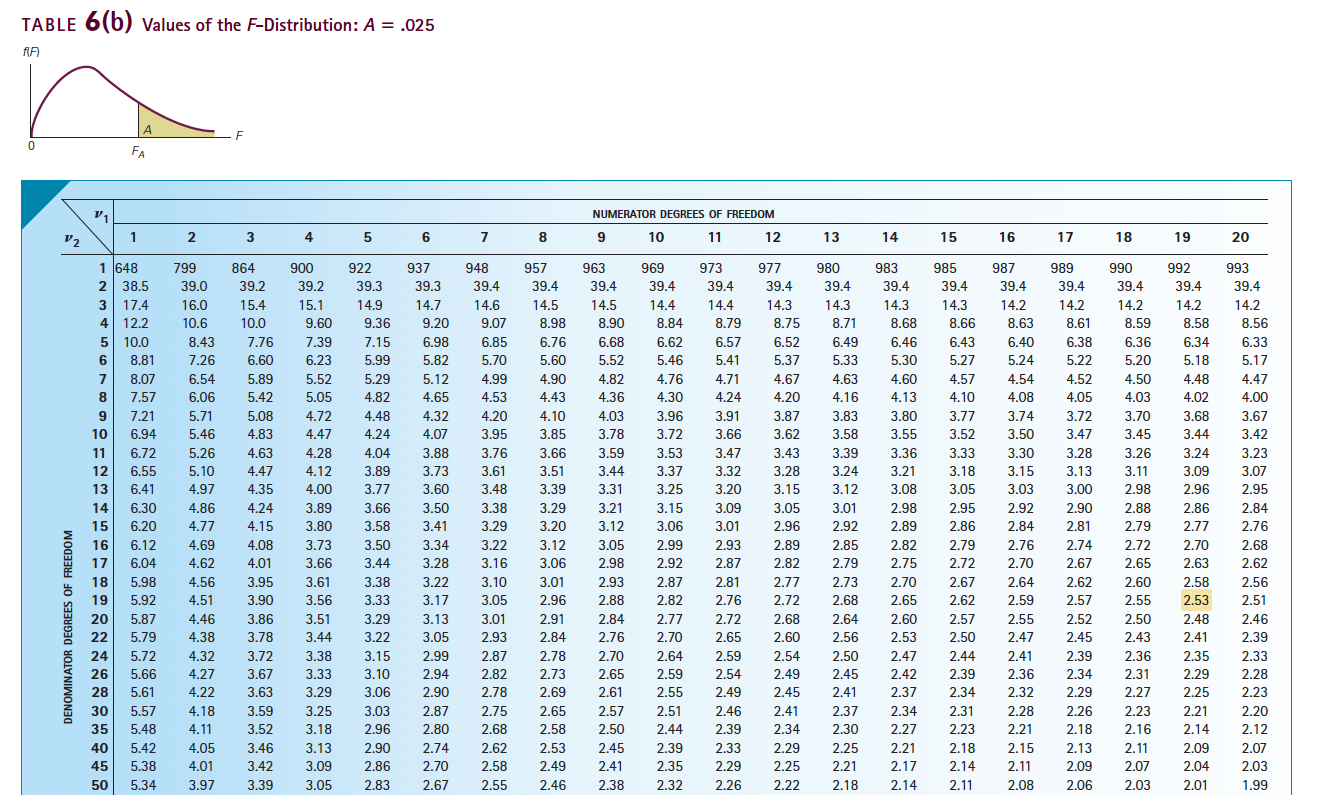
\includegraphics[width=11cm]{fstat2.png}	

	\end{frame}
	\begin{frame}
		\frametitle{Example}
		\framesubtitle{Testing $\mu_1 - \mu_2$ when $\sigma_1^2 = \sigma_2^2$}
		
		\begin{itemize}[label={\color{blue}$\blacktriangleright$}]
			\item Use the output to assess if there is a significant difference between the average weights of the two types of containers.
			\item Hypotheses:
			\[
			\begin{aligned}
				H_0 &: \mu_1 - \mu_2 = 0 \\
				H_1 &: \mu_1 - \mu_2 \neq 0
			\end{aligned}
			\]
		\end{itemize}
		
	\end{frame}
	\begin{frame}
		\frametitle{Example}
		\framesubtitle{Testing $\mu_1 - \mu_2$ when $\sigma_1^2 = \sigma_2^2$}
		
		\begin{itemize}[label={\color{blue}$\blacktriangleright$}]
			\item Test statistic:
			\begin{itemize}[label={\color{blue}$\blacktriangleright$}]
				\item First calculate the pooled sample variance:
				\[
				\begin{aligned}
					s_p^2 &= \frac{(n_1 - 1)s_1^2 + (n_2 - 1)s_2^2}{n_1 + n_2 - 2} \\[1ex]
					&= \frac{19 \times 31.26^2 + 19 \times 23.20^2}{20 + 20 - 2} \\[1ex]
					&= 757.7138
				\end{aligned}
				\]
			\end{itemize}
		\end{itemize}
		
	\end{frame}
	\begin{frame}
		\frametitle{Example}
		\framesubtitle{Testing $\mu_1 - \mu_2$ when $\sigma_1^2 = \sigma_2^2$}
		
		\begin{itemize}[label={\color{blue}$\blacktriangleright$}]
			\item Test statistic continued:
			\begin{itemize}[label={\color{blue}$\blacktriangleright$}]
				\item Then calculate the $T$-statistic:
				\[
				\begin{aligned}
					T &= \frac{(\overline{X}_1 - \overline{X}_2) - D_0}{\sqrt{s_p^2 \left(\frac{1}{n_1} + \frac{1}{n_2}\right)}} \\[2ex]
					&= \frac{(183.36 - 196.41) - 0}{\sqrt{757.7138 \times \left(\frac{1}{20} + \frac{1}{20}\right)}} \\[2ex]
					&= -1.4992
				\end{aligned}
				\]
			\end{itemize}
		\end{itemize}
		
	\end{frame}
	\begin{frame}
		\frametitle{Example}
		\framesubtitle{Testing $\mu_1 - \mu_2$ when $\sigma_1^2 = \sigma_2^2$}
		
		\begin{itemize}[label={\color{blue}$\blacktriangleright$}]
			\item Decision rule:
			\begin{itemize}[label={\color{blue}$\blacktriangleright$}]
				\item Compare to a $t$-distribution with $n_1 + n_2 - 2 = 38$ degrees of freedom.
				\item Since $t$-table doesn't list 38 degrees of freedom, use the closest in the table, i.e., 40.
				\item For $\alpha = 5\%$, rejection region is $T > 2.021$ or $T < -2.021$ (two-tailed test).
			\end{itemize}
			\item Conclusion:
			\begin{itemize}[label={\color{blue}$\blacktriangleright$}]
				\item Since $-2.021 < -1.4992 < 2.021$, there is insufficient evidence to reject the null hypothesis.
				\item That is, we conclude that the average weights of the two types of containers are the same.
			\end{itemize}
		\end{itemize}
		
	\end{frame}
		\begin{frame}
				\vspace{1cm}
			\centering
			{\color{blue}\large Paired Samples}
			
				\end{frame}
	\begin{frame}
		\frametitle{Paired Samples}
		
		\begin{itemize}[label={\color{blue}$\blacktriangleright$}]
			\item Paired samples are much easier to deal with than independent samples.
			
			\item Let $\{X_{11}, X_{12}, \ldots, X_{1n}\}$ and $\{X_{21}, X_{22}, \ldots, X_{2n}\}$ denote our two paired samples.
			
			\item For each pair of observations, calculate the difference $X_{Di} = X_{1i} - X_{2i}$, for $i = 1, \ldots, n$.
			
			\item We are now making inferences about $\mu_D = E(X_D)$, the population mean of these differences $X_{Di}$, and we are in a one-sample situation!
		\end{itemize}
		
	\end{frame}
	\begin{frame}
		\frametitle{Hypotheses and Test Statistic}
		
		\begin{itemize}[label={\color{blue}$\blacktriangleright$}]
			\item Hypotheses:
			\[
			\begin{aligned}
				H_0 &: \mu_D = D_0 \\
				H_1 &: \mu_D (\neq, <, >) D_0
			\end{aligned}
			\]
			
			\item Test statistic:
			\[
			T = \frac{\overline{X}_D - \mu_D}{\frac{s_D}{\sqrt{n}}} = \frac{\overline{X}_D - D_0}{\frac{s_D}{\sqrt{n}}}
			\]
			
			\item $\overline{X}_D$ and $s_D$ are the sample mean and sample standard deviation, respectively, of the paired differences.
		\end{itemize}
		
	\end{frame}
	\begin{frame}
		\frametitle{Decision Rule and Conclusion}
		
		\begin{itemize}[label={\color{blue}$\blacktriangleright$}]
			\item Decision rule:
			\begin{itemize}[label={\color{blue}$\blacktriangleright$}]
				\item We need to compare this $T$-statistic to a $t$-distribution with $n - 1$ degrees of freedom.
				\item Look up the $t$-table to determine rejection regions.
			\end{itemize}
			\item Conclusion:
			\begin{itemize}[label={\color{blue}$\blacktriangleright$}]
				\item If the $T$-statistic falls in the rejection region, reject $H_0$. Otherwise, fail to reject $H_0$.
			\end{itemize}
		\end{itemize}
		
	\end{frame}
	\begin{frame}
		\frametitle{Confidence Interval}
		
		\begin{itemize}[label={\color{blue}$\blacktriangleright$}]
			\item A $100(1 - \alpha)\%$ confidence interval for $\mu_D$, the population mean of the paired differences, is given by:
			
			\vspace{0.5cm}
			
			\[
			\overline{X}_D \pm t_{\frac{\alpha}{2},n-1} \frac{s_D}{\sqrt{n}}
			\]
		\end{itemize}
		
	\end{frame}
\begin{frame}
	\frametitle{Example}
	
	\begin{itemize}[label={\color{blue}$\blacktriangleright$}]
		\item As a test of how effective antilock brakes are, a car buyer hit the brakes and, using a stopwatch, recorded the number of seconds it took to stop an ABS-equipped car and another identical car without ABS.
		
		\item The speeds (mph) when the brakes were applied and the number of seconds each car took to stop are listed on the next slide.
		
		\item Can we infer that ABS is better?
	\end{itemize}
	
\end{frame}
\begin{frame}
	\frametitle{Example}
	
	\begin{center}
		\begin{tabular}{ccccccccc}
			\toprule
			Speeds & 20 & 25 & 30 & 35 & 40 & 45 & 50 & 55 \\
			\midrule
			ABS & 3.6 & 4.1 & 4.8 & 5.3 & 5.9 & 6.3 & 6.7 & 7.0 \\
			Non-ABS & 3.4 & 4.0 & 5.1 & 5.5 & 6.4 & 6.5 & 6.9 & 7.3 \\
			\midrule
			Difference & 0.2 & 0.1 & $-$0.3 & $-$0.2 & $-$0.5 & $-$0.2 & $-$0.2 & $-$0.3 \\
			\bottomrule
		\end{tabular}
	\end{center}
	
	\end{frame}
	\begin{frame}
		\frametitle{Example}
		
		\begin{itemize}[label={\color{blue}$\blacktriangleright$}]
			\item Hypotheses:
			\[
			\begin{aligned}
				H_0 &: \mu_D = 0 \\
				H_1 &: \mu_D < 0
			\end{aligned}
			\]
			
			\item From the differences calculated in the previous table, we can obtain their sample mean and sample standard deviation, $\overline{X}_D = -0.175$ and $s_D = 0.2252$.
		\end{itemize}
		
	\end{frame}
	\begin{frame}
		\frametitle{Example}
		
		\begin{itemize}[label={\color{blue}$\blacktriangleright$}]
			\item Test statistic:
			\[
			T = \frac{\overline{X}_D - D_0}{\frac{s_D}{\sqrt{n}}} = \frac{-0.175 - 0}{\frac{0.2252}{\sqrt{8}}} = -2.1980
			\]
			
			\item Decision rule and conclusion:
			\begin{itemize}[label={\color{blue}$\blacktriangleright$}]
				\item Rejection region is $T < t_{0.05,7} = -1.895$.
				\item Since $-2.1980 < -1.895$, we reject $H_0$.
				\item That is, there is enough evidence to infer that ABS is better.
			\end{itemize}
		\end{itemize}
		
	\end{frame}
	\begin{frame}
		\frametitle{Why Product of F-Distribution Critical Values Equals 1}
		
		\begin{itemize}[label={\color{blue}$\blacktriangleright$}]
			\item Let $F_\alpha(df_1, df_2)$ be the upper $\alpha$ critical value of $F(df_1, df_2)$
			\item We want to prove: $F_\alpha(df_1, df_2) \cdot F_{1-\alpha}(df_2, df_1) = 1$
		\end{itemize}
			\end{frame}
	\begin{frame}
	\frametitle{Why Product of F-Distribution Critical Values Equals 1}
			\begin{align*}
				&\text{If } X \sim F(df_1, df_2), \text{ then } \frac{1}{X} \sim F(df_2, df_1) \\[1ex]
				&P(X > F_\alpha(df_1, df_2)) = \alpha \\[1ex]
				&P\left(\frac{1}{X} < \frac{1}{F_\alpha(df_1, df_2)}\right) = \alpha \\[1ex]
				&\frac{1}{F_\alpha(df_1, df_2)} = F_{1-\alpha}(df_2, df_1) \\[1ex]
				&\therefore F_\alpha(df_1, df_2) \cdot F_{1-\alpha}(df_2, df_1) = 1
			\end{align*}
		
	\end{frame}
	
	\begin{frame}
		\vspace{1cm}
		\centering
		{\color{blue}\large Test sample proportion}
		
	\end{frame}
	\begin{frame}
		\frametitle{Testing $p_1 - p_2$}
		
		\begin{itemize}[label={\color{blue}$\blacktriangleright$}]
			\item Just as with means, we can test the difference between two population proportions.
			
			\item We typically require \emph{independent} samples when dealing with proportions.
			
			\item We are making inferences about $p_1 - p_2$, so what is a reasonable estimator of $p_1 - p_2$?
			
			\item We can use $\hat{p}_1 - \hat{p}_2$ as an estimator of $p_1 - p_2$, where $\hat{p}_1 = \frac{X_1}{n_1}$ and $\hat{p}_2 = \frac{X_2}{n_2}$.
		\end{itemize}
		
	\end{frame}
	\begin{frame}
		\frametitle{Testing $p_1 - p_2$}
		
		\begin{itemize}[label={\color{blue}$\blacktriangleright$}]
			\item For large $n_1$ and $n_2$, the sampling distribution of $\hat{p}_1 - \hat{p}_2$ is approximately normal with mean and variance given by:
			
			\vspace{0.5cm}
			
			\[
			E(\hat{p}_1 - \hat{p}_2) = p_1 - p_2
			\]
			\[
			V(\hat{p}_1 - \hat{p}_2) = \frac{p_1(1-p_1)}{n_1} + \frac{p_2(1-p_2)}{n_2}
			\]
			
			\vspace{0.5cm}
			
			\item As a rule of thumb, this normal approximation is valid provided $n_1p_1$, $n_1(1-p_1)$, $n_2p_2$ and $n_2(1-p_2)$ are all larger than 5.
		\end{itemize}
		
	\end{frame}
	\begin{frame}
		\frametitle{Testing $p_1 - p_2$}
		
		\begin{itemize}[label={\color{blue}$\blacktriangleright$}]
			\item Hypotheses:
			\[
			\begin{aligned}
				H_0 &: p_1 - p_2 = D_0 \\
				H_1 &: p_1 - p_2 (\neq, <, >) D_0
			\end{aligned}
			\]
			for some $D_0 \neq 0$.
			
			\item Test statistic:
			\[
			Z = \frac{(\hat{p}_1 - \hat{p}_2) - (p_1 - p_2)}{\sqrt{\frac{\hat{p}_1(1-\hat{p}_1)}{n_1} + \frac{\hat{p}_2(1-\hat{p}_2)}{n_2}}} = \frac{(\hat{p}_1 - \hat{p}_2) - D_0}{\sqrt{\frac{\hat{p}_1(1-\hat{p}_1)}{n_1} + \frac{\hat{p}_2(1-\hat{p}_2)}{n_2}}}
			\]
		\end{itemize}
		
	\end{frame}
	\begin{frame}
		\frametitle{Testing $p_1 - p_2$}
		
		\begin{itemize}[label={\color{blue}$\blacktriangleright$}]
			\item What happens when $D_0 = 0$?
			
			\item Hypotheses:
			\[
			\begin{aligned}
				H_0 &: p_1 - p_2 = 0 \\
				H_1 &: p_1 - p_2 (\neq, <, >) 0
			\end{aligned}
			\]
			
			\item We have to change the test statistic slightly.
		\end{itemize}
		
	\end{frame}
	\begin{frame}
		\frametitle{Testing $p_1 - p_2$}
		
		\begin{itemize}[label={\color{blue}$\blacktriangleright$}]
			\item Test statistic:
			\[
			Z = \frac{(\hat{p}_1 - \hat{p}_2) - (p_1 - p_2)}{\sqrt{\hat{p}(1 - \hat{p})\left(\frac{1}{n_1} + \frac{1}{n_2}\right)}} = \frac{(\hat{p}_1 - \hat{p}_2) - 0}{\sqrt{\hat{p}(1 - \hat{p})\left(\frac{1}{n_1} + \frac{1}{n_2}\right)}}
			\]
			
			where $\hat{p}$ is the \textbf{combined proportion}:
			
			\[
			\hat{p} = \frac{X_1 + X_2}{n_1 + n_2} = \frac{n_1\hat{p}_1 + n_2\hat{p}_2}{n_1 + n_2}
			\]
		\end{itemize}
		
	\end{frame}
	\begin{frame}
		\frametitle{Confidence Interval for $p_1 - p_2$}
		
		\begin{itemize}[label={\color{blue}$\blacktriangleright$}]
			\item A $100(1 - \alpha)\%$ confidence interval for $p_1 - p_2$ is given by:
			
			\vspace{0.5cm}
			
			\[
			(\hat{p}_1 - \hat{p}_2) \pm z_{\frac{\alpha}{2}} \sqrt{\frac{\hat{p}_1(1 - \hat{p}_1)}{n_1} + \frac{\hat{p}_2(1 - \hat{p}_2)}{n_2}}
			\]
			
			\vspace{0.5cm}
			
			\item Note that we can't assume the population proportions are equal when constructing the confidence interval.
		\end{itemize}
		
	\end{frame}
	\begin{frame}
		\frametitle{Example}
		
		\begin{itemize}[label={\color{blue}$\blacktriangleright$}]
			\item These statistics are calculated from samples taken from two Bernoulli populations:
			
			\vspace{0.5cm}
			
			\[
			\hat{p}_1 = 0.6, \quad n_1 = 225, \quad \hat{p}_2 = 0.55, \quad n_2 = 225
			\]
			
			\vspace{0.5cm}
			
			\item Calculate the $p$-value of a test to determine whether there is evidence to infer that the population proportions differ.
		\end{itemize}
		
	\end{frame}
	\begin{frame}
		\frametitle{Hypotheses and Test Statistic}
		
		\begin{itemize}[label={\color{blue}$\blacktriangleright$}]
			\item Hypotheses:
			\[
			\begin{aligned}
				H_0 &: p_1 - p_2 = 0 \\
				H_1 &: p_1 - p_2 \neq 0
			\end{aligned}
			\]
			
			\item Test statistic:
			\begin{itemize}[label={\color{blue}$\blacktriangleright$}]
				\item Combined proportion:
				\[
				\hat{p} = \frac{n_1\hat{p}_1 + n_2\hat{p}_2}{n_1 + n_2} = \frac{225 \times 0.6 + 225 \times 0.55}{225 + 225} = 0.575
				\]
			\end{itemize}
		\end{itemize}
		
	\end{frame}
	\begin{frame}
		\frametitle{Test Statistic}
		
		\begin{itemize}[label={\color{blue}$\blacktriangleright$}]
			\item Test statistic continued:
			\begin{itemize}[label={\color{blue}$\blacktriangleright$}]
				\item $Z$-statistic:
				\[
				\begin{aligned}
					Z &= \frac{(\hat{p}_1 - \hat{p}_2) - 0}{\sqrt{\hat{p}(1 - \hat{p}) \left(\frac{1}{n_1} + \frac{1}{n_2}\right)}} \\
					&= \frac{0.6 - 0.55}{\sqrt{0.575(1 - 0.575) \left(\frac{1}{225} + \frac{1}{225}\right)}} \\
					&= 1.0728
				\end{aligned}
				\]
			\end{itemize}
		\end{itemize}
		
	\end{frame}
\begin{frame}
	\frametitle{Decision Rule and Conclusion}
	
	\begin{itemize}[label={\color{blue}$\blacktriangleright$}]
		\item Decision rule
		\begin{itemize}[label={\color{blue}$\blacktriangleright$}]
			\item The $p$-value is given by:
			\[
			\begin{aligned}
				p\text{-value} &= P(Z < -1.07) + P(Z > 1.07) \\
				&= 2 \times P(Z < -1.07) \\
				&= 0.2846
			\end{aligned}
			\]
		\end{itemize}
		
		\item Conclusion:
		\begin{itemize}[label={\color{blue}$\blacktriangleright$}]
			\item Since 0.2846 is greater than $\alpha = 0.05$ or even $\alpha = 0.1$, we would fail to reject the null hypothesis at both the 5\% and 10\% significance levels.
			\item We conclude the population proportions do not differ.
		\end{itemize}
	\end{itemize}
	
\end{frame}
\end{document}